\chapter{2048と完全解析}

\section{2048の完全解析とは}
\label{sec:solving}
2048は$1$人用のゲームであるため, 勝敗のようなプレイヤの明確な目標は存在しない.
そのためプレイヤが何を目標とするかによって, プレイヤの最善手の定義は変化する.
また\ref{sec:rule}節で述べたようにゲームはランダム性を伴うため, 同じ状態から毎回同じ手を選んでも結果は確率的に変動する.

そこで本稿ではある状態$s$における最善手を「$s$から獲得できる得点の合計の期待値が最も高くなるような手」と定義する.
これは多くの上手な人間やAIが2048のタイルを完成させることに留まらず, より多くの得点を獲得することを目標としていることから妥当な定義であると考えられる.
状態$s$から最善手を選び続けて獲得できる得点の合計の期待値を状態$s$の\textgt{価値}と呼び, $V(s)$で表すことにする.
このとき$V(s)$は式~\ref{eq:value}のように再帰的な形式で書くことができる.
ただし$r(s,a)$は状態$s$から行動$a$をとって獲得する得点, $s_\text{next} \in \mathcal{T}(s,a)$は状態$s$から行動$a$をとって遷移しうる次の状態の集合を表す~(図~\ref{fig:state_afterstate}を参照).

\begin{align}
    V(s) =
    \begin{cases}
        0 & (s \text{が終了状態}) \\
        \max_a \left(r(s,a) + \mathbb{E}_{s_\text{next} \in \mathcal{T}(s,a)} V(s_\text{next}) \right) & (\text{otherwise})
    \end{cases}
    \label{eq:value}
\end{align}

\begin{figure}[t]
    \centering
    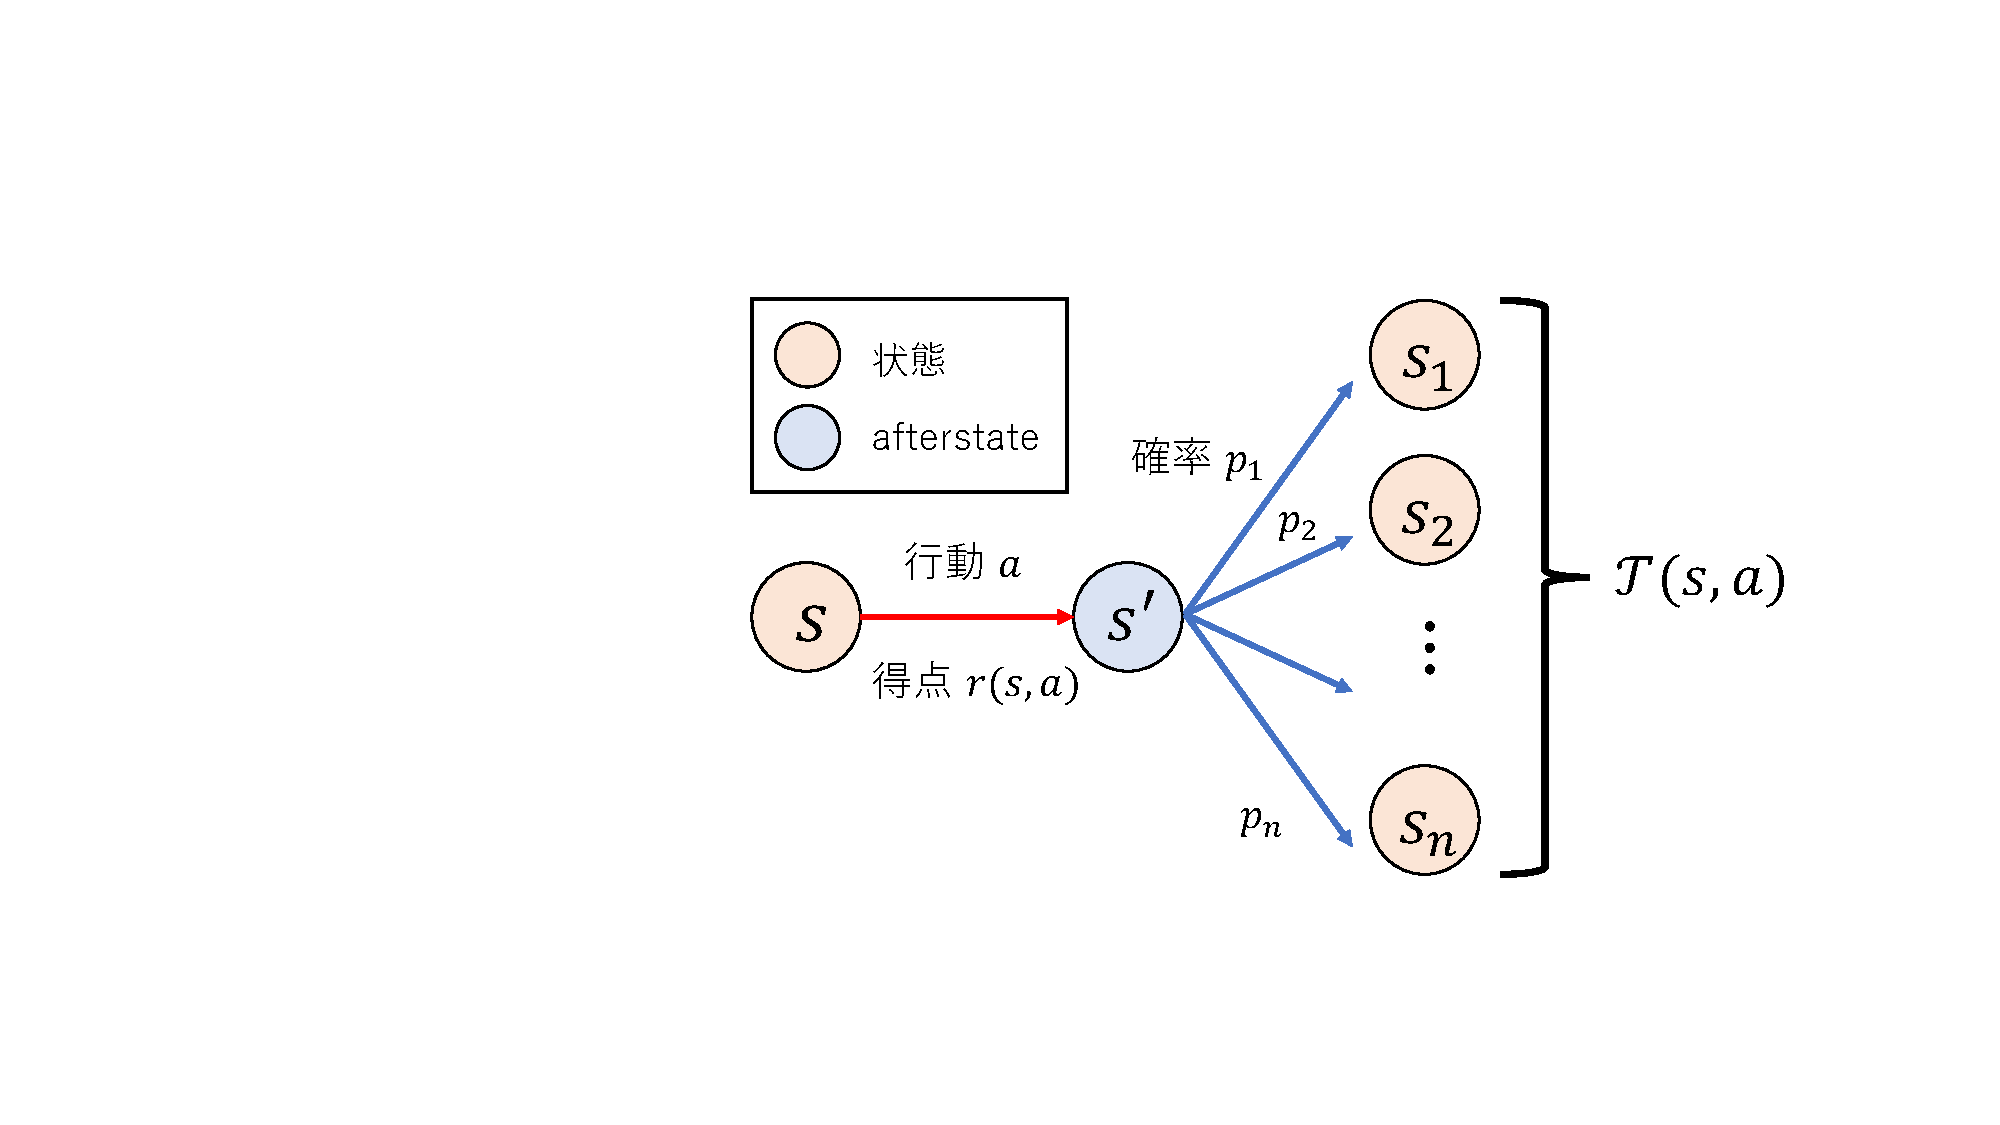
\includegraphics[width=\linewidth{}]{figures/state_afterstate.pdf}
    \caption{式~\ref{eq:value}の補足図 \label{fig:state_afterstate}}
\end{figure}

ゲームに現れうるすべての状態の価値を計算すれば, 任意の状態において最善手を選ぶことができる.
本稿ではこれを2048の完全解析ということにする.

完全解析によって, 最善手を選び続けるプレイヤの戦略やゲームの初期状態の価値を知りたい人は少なくないだろう.
また2048を対象とした強化学習の研究は数多くあり, 完全解析によってそれらの良し悪しを定量的に評価することができる.
一方で, 2048を完全解析することはそのゲーム木の大きさから現状難しいと考えられる.
そこで以降では本来$4\times4$盤面上で行われる2048のミニゲームとして, 盤面サイズを縮小した2048を完全解析することを考える.

\section{2048のミニゲームの完全解析}
\label{sec:mini2048}
本節の内容は文献~\cite{3x3_2048}および文献~\cite{4x3_2048}を元に執筆された.

基本的なルールは2048と同じで盤面サイズを$4\times4$から縮小したゲームを完全解析することを考える.
盤面サイズに関わらず2048の完全解析は以下の$2$つのステップに分けて行うことができる.

\begin{enumerate}
    \item ゲームに現れうるすべての状態の列挙
    \item 列挙した状態の価値の計算
\end{enumerate}

\ref{subsec:enumeration}節と~\ref{subsec:calculation}節で具体的な方法について述べる.

\subsection{幅優先探索によるすべての状態の列挙}
\label{subsec:enumeration}
まずゲームに現れうるすべての状態を列挙する.
これはキューを用いた幅優先探索によって行うことができる.

\subsection{後退解析による状態の価値の計算}
\label{subsec:calculation}
\ref{subsec:enumeration}節で列挙した状態の価値を後退解析によって計算する.